A hadron can be misidentified as a photon if fragmentation processes results in mainly neutral hadrons that subsequently decay to collimated pairs of photons.
The production of \zj\ where the \PZ\ boson decays to neutrinos is a high-rate process, and it mimicks the photon plus \met\ signature if the hadrons from the jet are misidentified.
We estimate the rate of misidentified hadrons in the signal region by reweighting a hadron proxy control sample by the ratio of the number of misidentified hadrons to the number of hadron proxy objects.
This procedure is shown in Figure~\ref{fig:hfake_diagram}.

\begin{figure}[htbp]
  \centering
  \resizebox{\textwidth}{!}{
    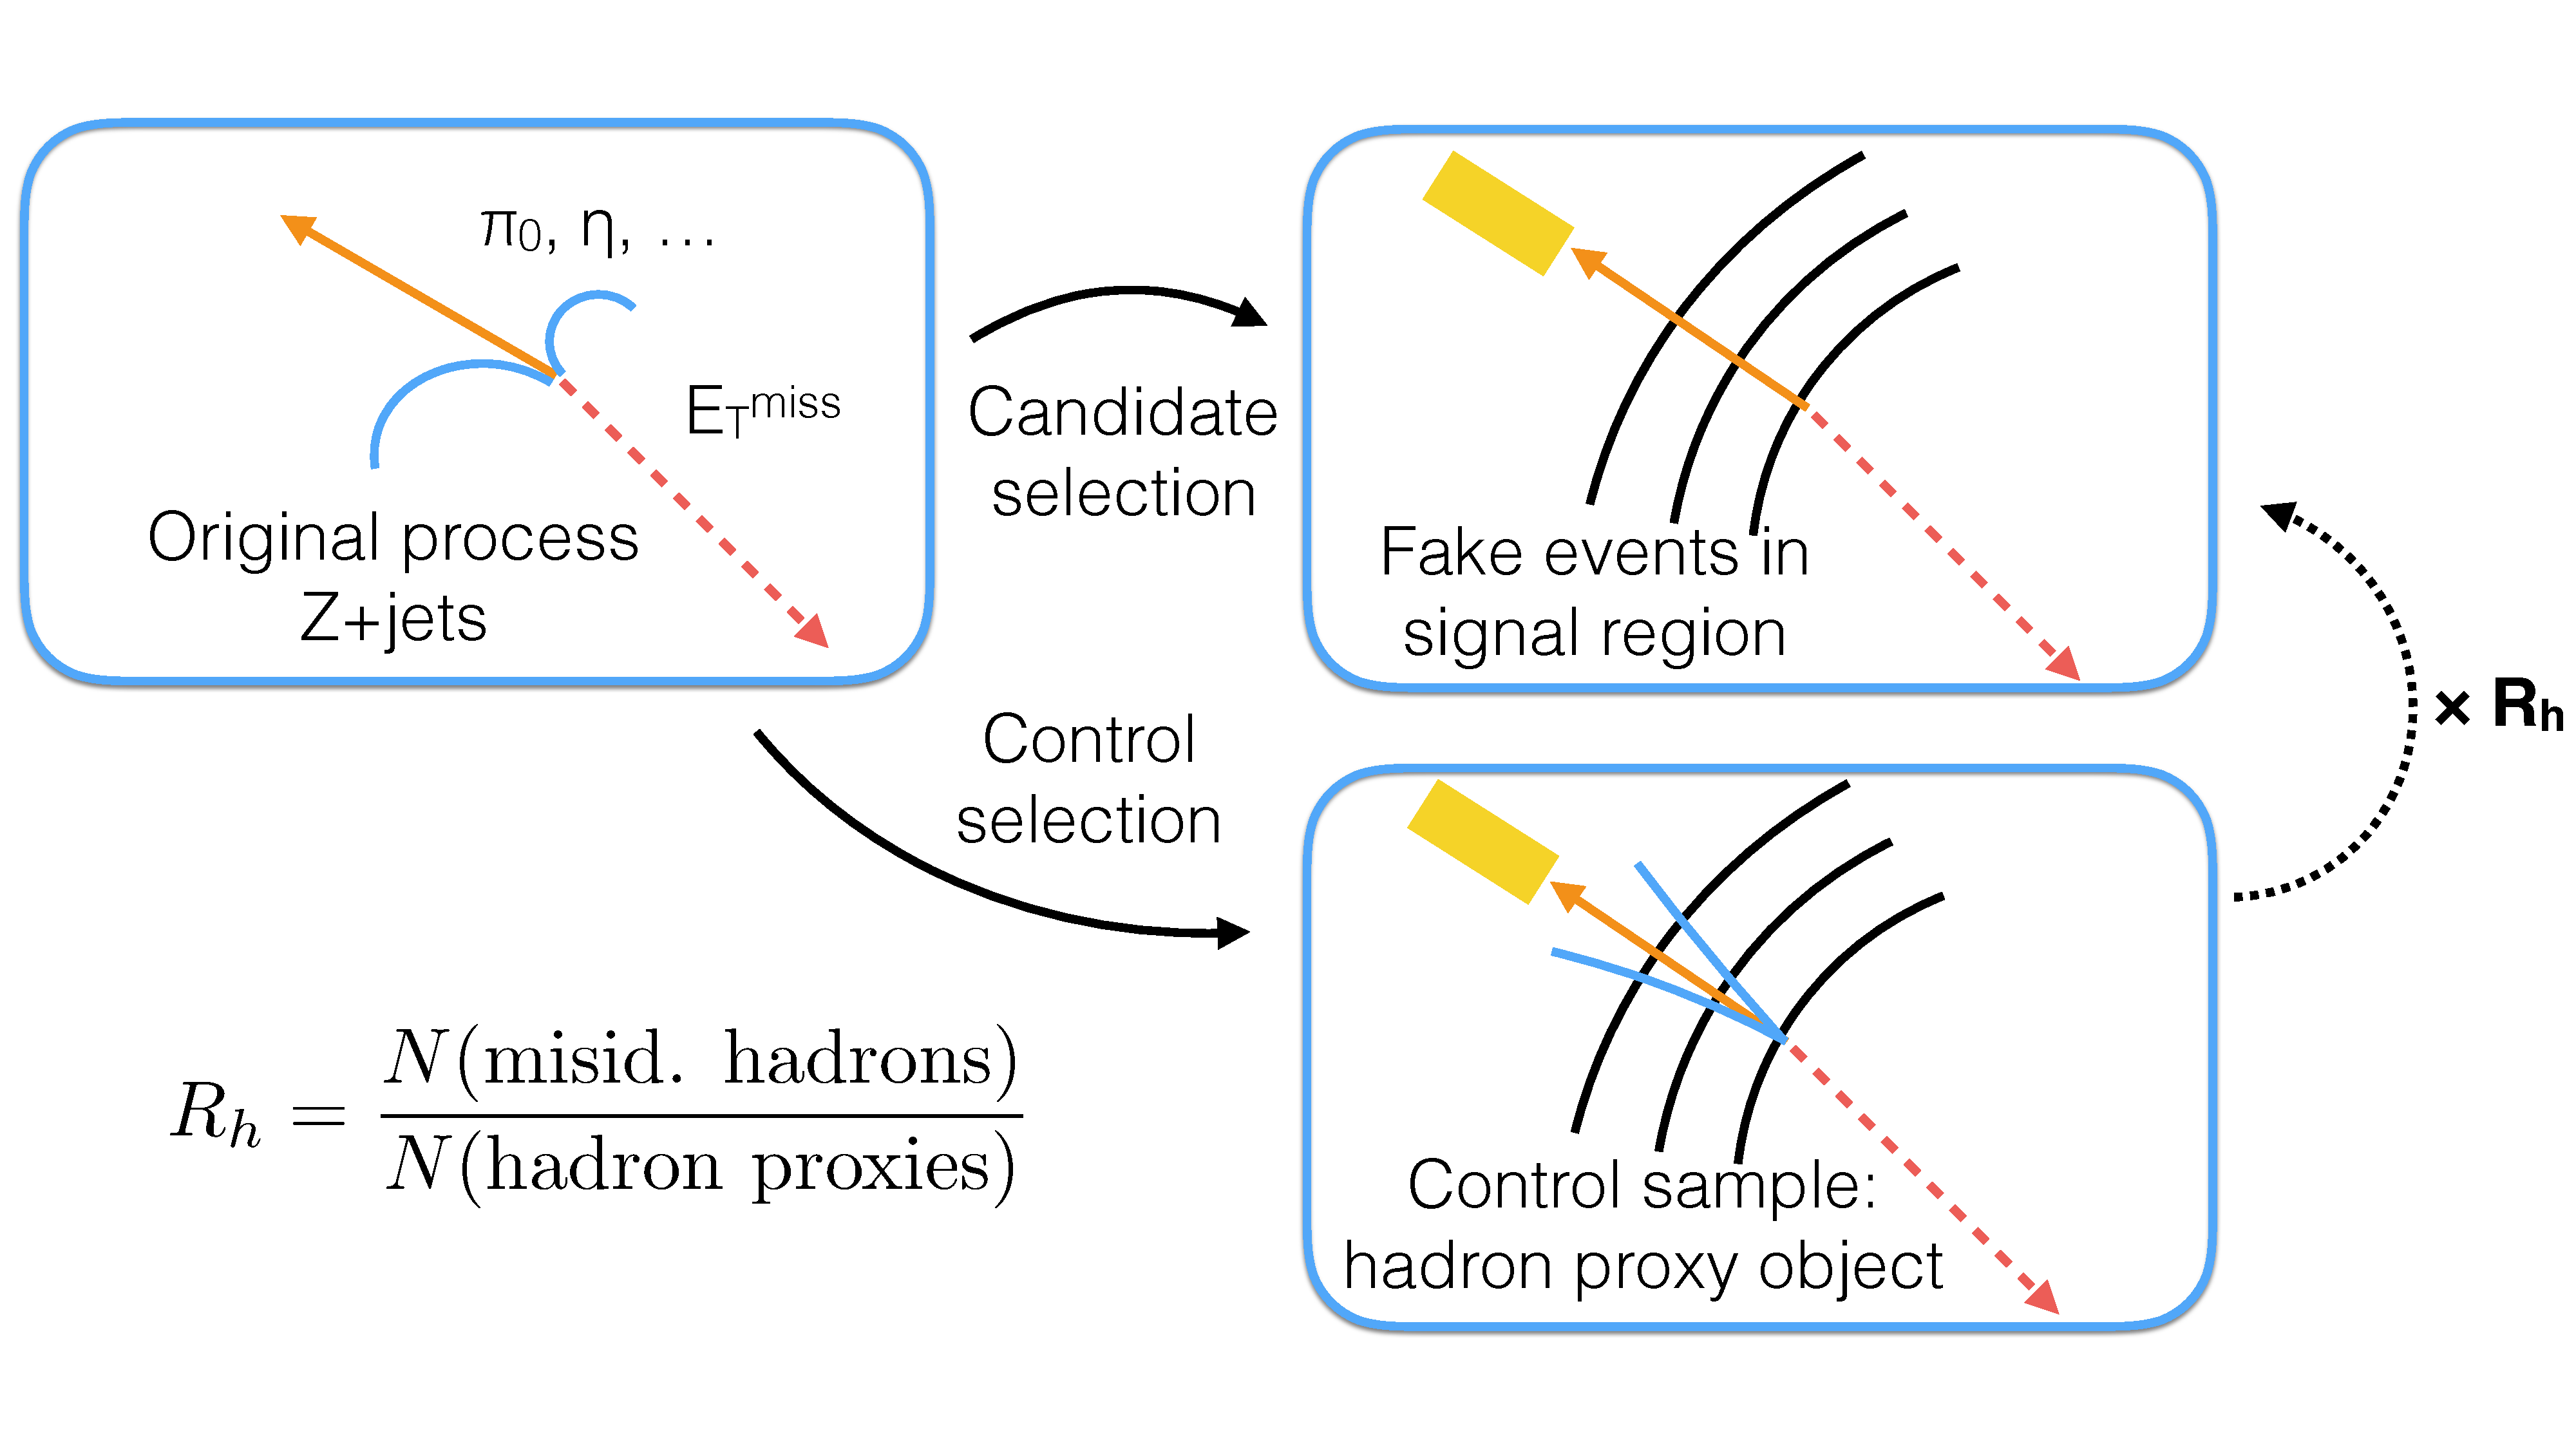
\includegraphics[]{Analysis/Figures/hfake/hfake_diagram.pdf}
  }
  \caption{
       Events where a jet recoils against a single \PZ\ boson decays to neutrinos mimic the photon plus \met\ signature if the hadrons from the jet are isolated. 
       The rate of misidentified hadrons in the signal region is estimated by reweighting a hadron proxy control sample by the ratio of the number of misidentified hadrons to the number of hadron proxy objects. 
    }
    \label{fig:hfake_diagram}
\end{figure}

\begin{figure}[htbp]
  \centering
  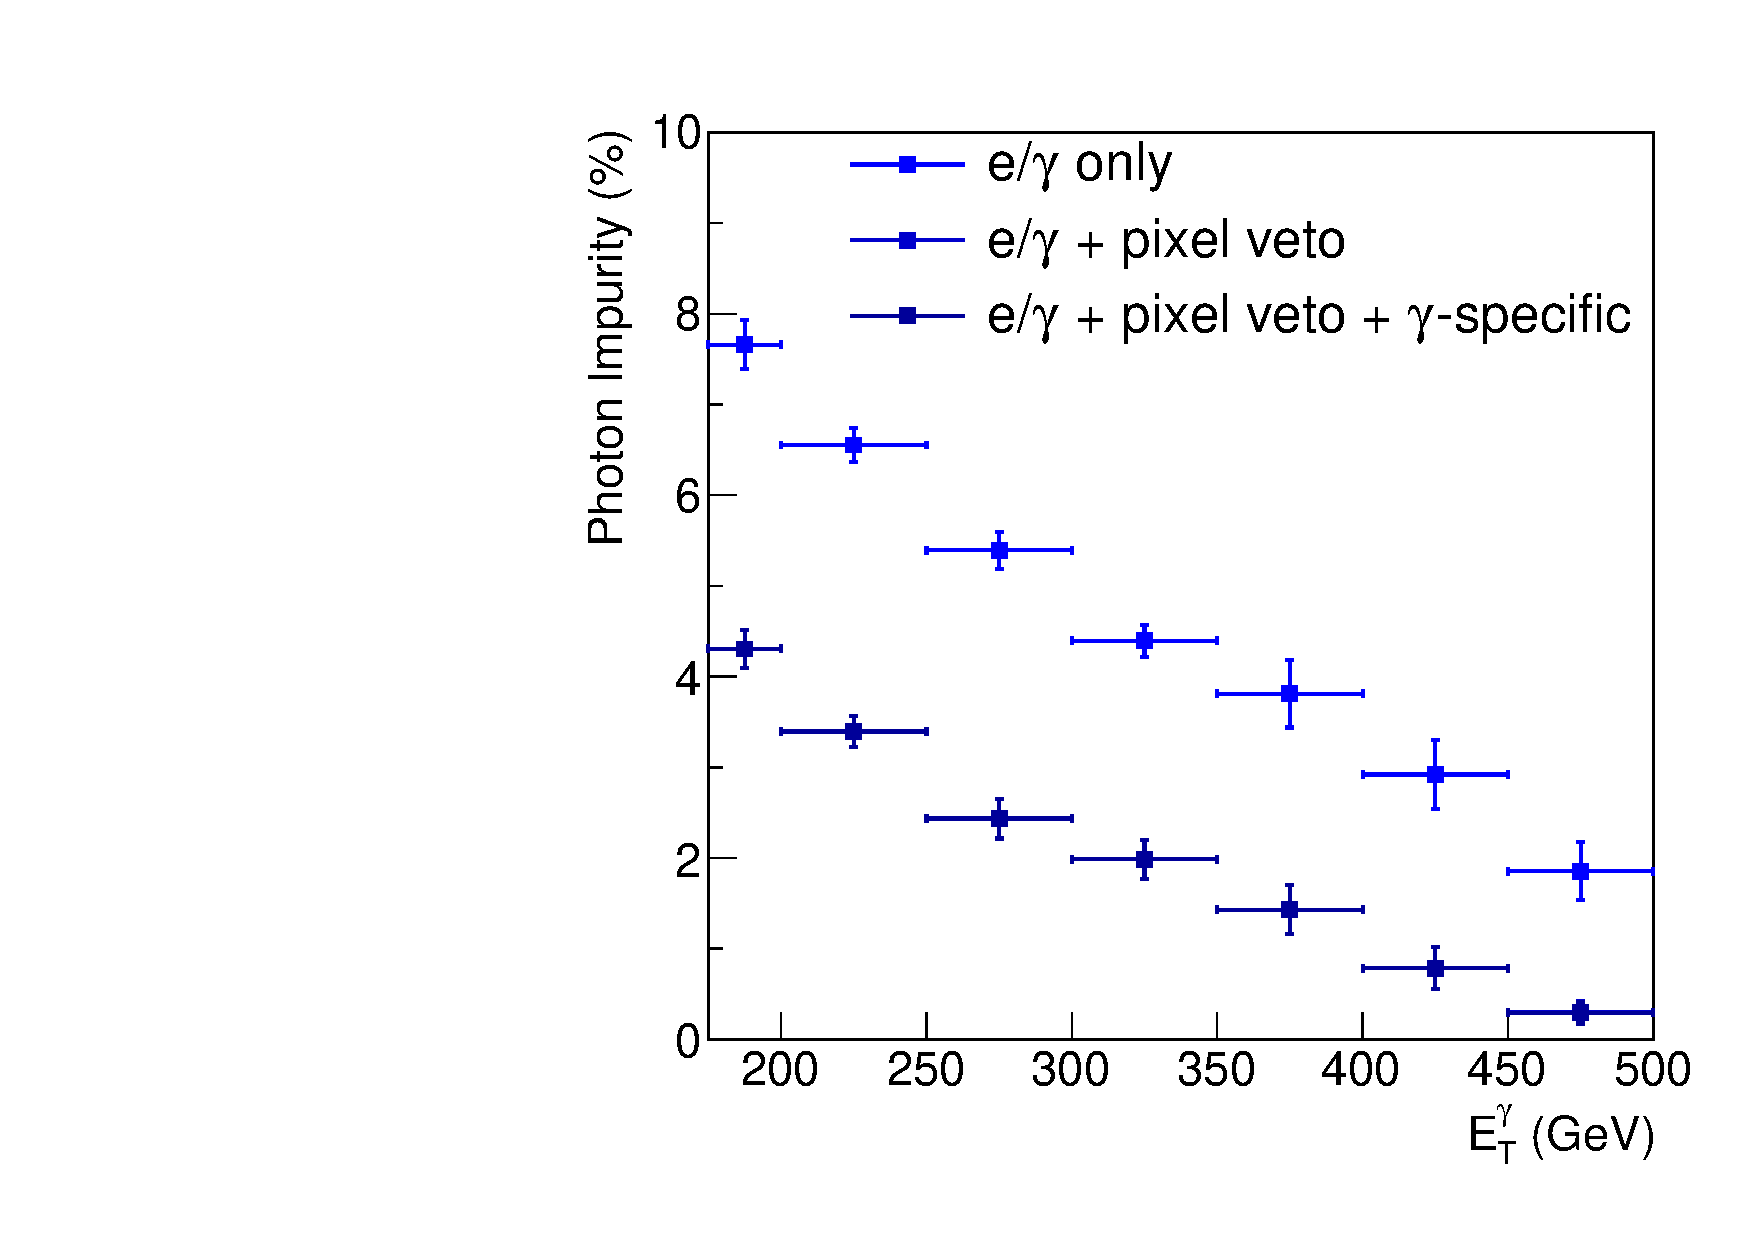
\includegraphics[width=0.5\textwidth]{Analysis/Figures/hfake/plot_impurity_barrel_medium.pdf}
  \caption{
    The percent impurity for photons as a function of \pt. 
    The different bands show the effects of adding different stages of the full ID, starting with the \egamma\ portion of the ID and successively adding the pixel seed veto followed by the rest of the \Pgg-specific portion of the ID.
    These last two curves overlap, as the non-collision rejection cuts do not effect the rate at which hadrons are misidentified as photons.
  }
  \label{fig:impurity-compsb}
\end{figure}

Without the presence of additional charged tracks or neutral hadron energy deposits, the only way to distinguish EM-like hadrons from real photons is through the shower shape. 
Thus, we measure the fraction of hadronic objects within the pool of photon candidate objects in the EM object+jet measurement sample defined in Table~\ref{tab:emjet} using the \sieie\ template fit method from Section~\ref{sec:pvsf}.
Figure~\ref{fig:impurity-compsb} and Table~\ref{tab:hfake-impurity-systs} show the final impurity and associated uncertainties as a function of \pt. 

\begin{table}[htbp]
  \centering
  \begin{tabular}{ c|c|c c c c }
    \pt & Nominal & \multicolumn{4}{ |c }{Sources of Systematic Uncertainty} \\
    (GeV) & (\%) & Sideband & CH Iso Shape & Signal Shape & Bgkd. Stats \\
    \hline
    (175, 200)  & $4.31 \pm 0.21$ & 0.09 & 0.18 & 0.05 & 0.04 \\
    (200, 250)  & $3.39 \pm 0.17$ & 0.01 & 0.16 & 0.06 & 0.03 \\
    (250, 300)  & $2.44 \pm 0.22$ & 0.14 & 0.16 & 0.06 & 0.05 \\
    (300, 350)  & $1.99 \pm 0.23$ & 0.12 & 0.16 & 0.07 & 0.08 \\
    (350, 400)  & $1.43 \pm 0.28$ & 0.23 & 0.11 & 0.05 & 0.10 \\
    (400, $\infty$)  & $0.63 \pm 0.30$ & 0.27 & 0.09 & 0.05 & 0.05 \\
  \end{tabular}
  \caption{Impurities for photons as a function of \pt.}
  \label{tab:hfake-impurity-systs}
\end{table}

The hadron-to-photon misidentification rate $R_h$ is obtained by dividing the estimated number of misidentified hadrons in the EM object+jet measurement sample by the number of events in a hadron proxy+jet control sample.
This control sample is obtained by requiring a hadron proxy object with $\ET > 175\GeV$ and $\abs\eta < 1.44$ plus at least one jet with $\pt > 100\GeV$ and $\abs\eta < 2.5$ which passes the loose jet ID. 
An hadron proxy object is a photon candidate that passes the the \egamma\ and \Pgg-specific IDs with the following inverted cut:  $\ICH > 1.146\GeV$.
We use \ICH\ instead of \ICHmax\ since the presence of a high-\pt\ jet guarantees we have chosen the correct primary vertex.
Additionally, we apply an $\met < 60\GeV$ cut to make this region orthogonal to the signal region.
Table~\ref{tab:proxyjet} summarizes the selections for the hadron proxy+jet control sample. 

\begin{table}[htbp]
  \centering
    \begin{tabular}{l | l | r}
      Variable & Selection & Motivation \\
      \hline
      $\ET$ & $ > 175\GeV$ & hadron proxy object passing trigger \\
      $\abs{\eta}$ & $ < 1.44$ & match signal region kinematics \\
      \egamma\ ID & Pass all but \ICHmax\ & must be photon-like \\
      \Pgg-specific ID & Pass & must be photon-like \\ 
      \ICH\ &  $ > 1.146\GeV$ & inverted to mimic hadrons \\
      $\pt^j$ & $> 100\GeV$ & match EM object+jet sample kinematics \\
      $\abs{\eta^j}$ & $ < 2.5$ & match EM object+jet sample kinematics \\
      Loose Jet ID & Pass & match EM object+jet sample kinematics \\
      $\met $ & $ < 60\GeV$ & match EM object+jet sample kinematics \\
    \end{tabular}
  \caption{Selections for the hadron proxy+jet control sample.}
  \label{tab:proxyjet}
\end{table}

Additional tight and loose hadron proxy objects and control samples are made by tightening and loosening the constant term in the \INH\ and \Ig\ requirements on the proxy object.
The specific values for each proxy object are shown in Table~\ref{tab:hadron_proxy}. 

\begin{table}[htbp]
  \centering
    \begin{tabular}{l | r | r}
      & \INH\ (\GeVns)& \Ig\ (\GeVns) \\
      \hline
      Nominal & 2.792 & 2.176 \\ 
      Loose & 10.910 & 3.630 \\
      Tight & 0.264 & 2.362 
    \end{tabular}
  \caption{Constant terms in the \INH\ and \Ig\ selections for the hadron proxy objects.}
  \label{tab:hadron_proxy}
\end{table}

Figure~\ref{fig:hadronTFactor} shows the derived $R_{h}$ factor as a function of \ET\ along with the various distributions used for its derivation.

\begin{figure}[htbp]
  \centering
  \resizebox{0.91\textwidth}{!}{
    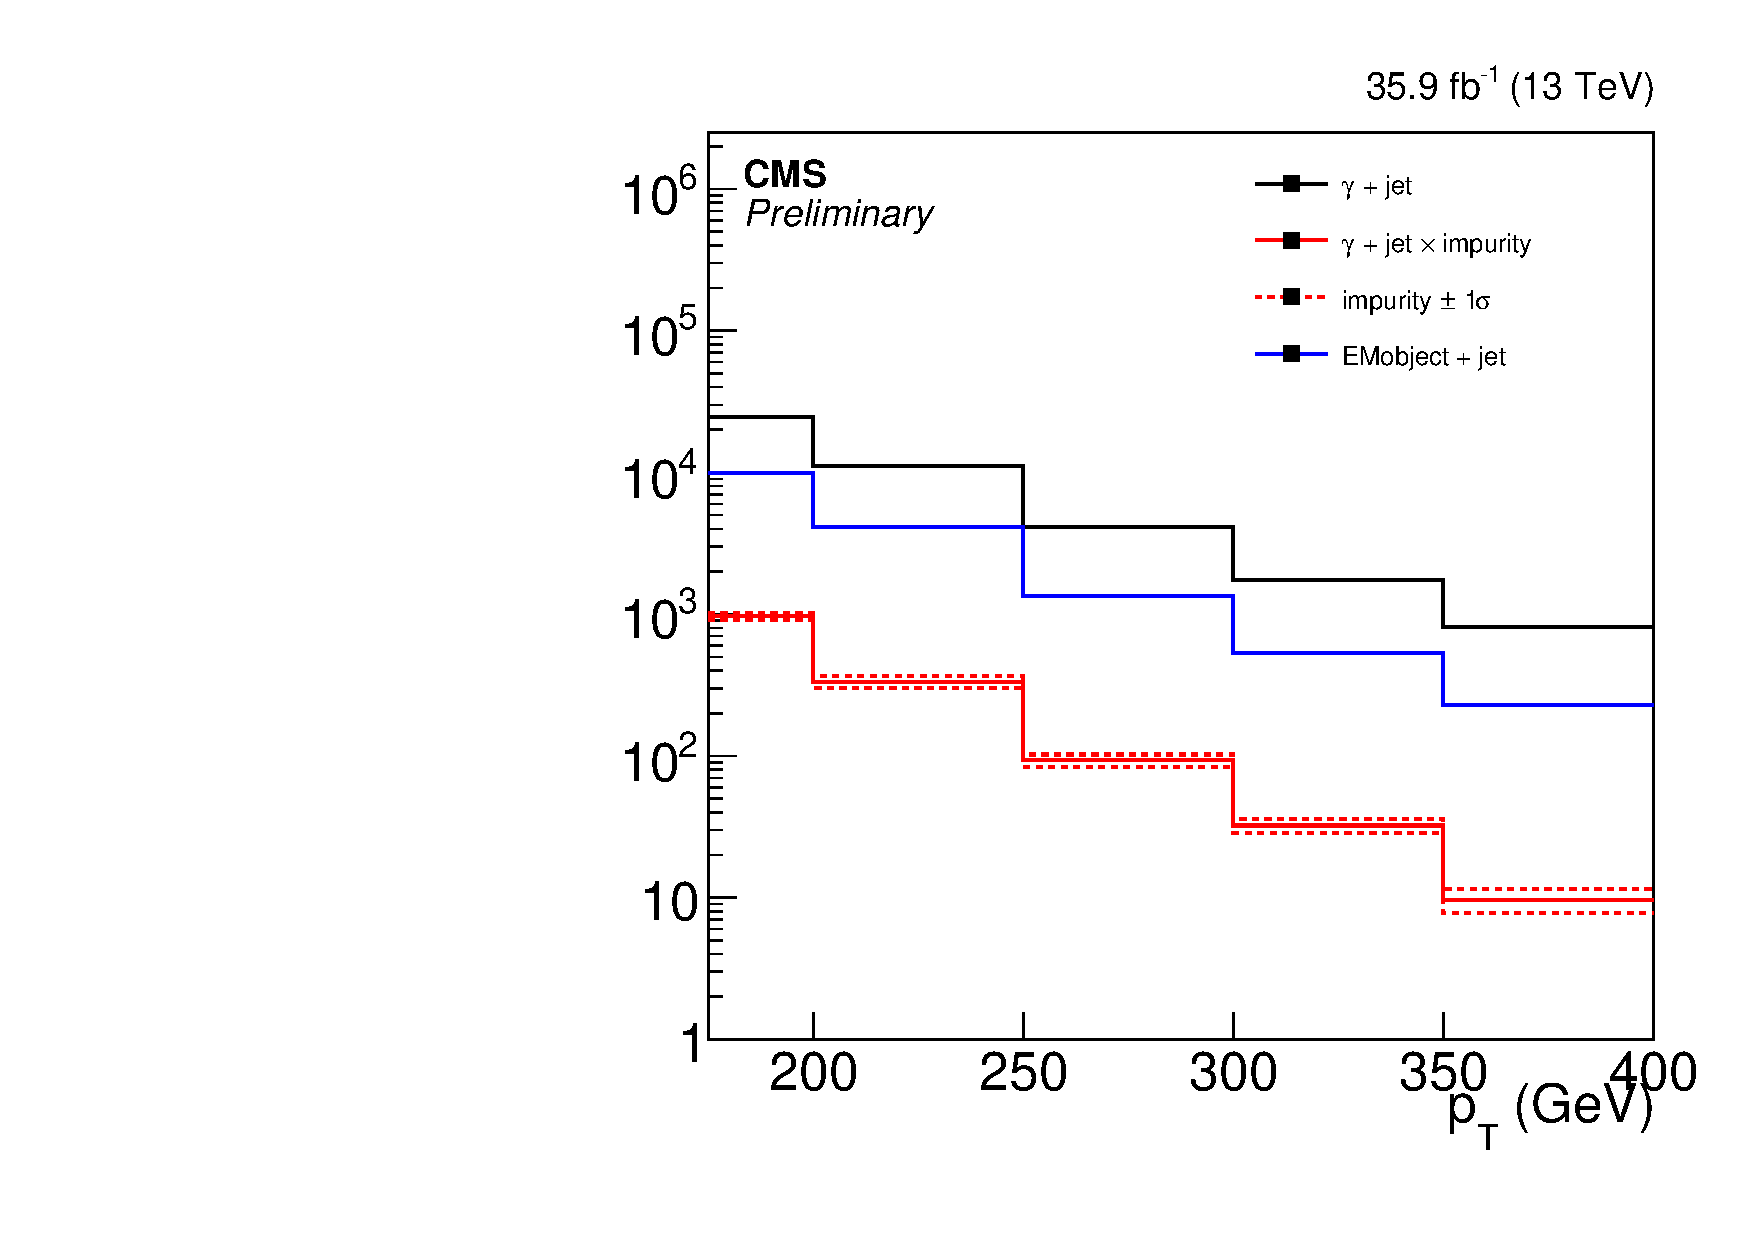
\includegraphics[]{Analysis/Figures/hfake/distributionsNom.pdf}
    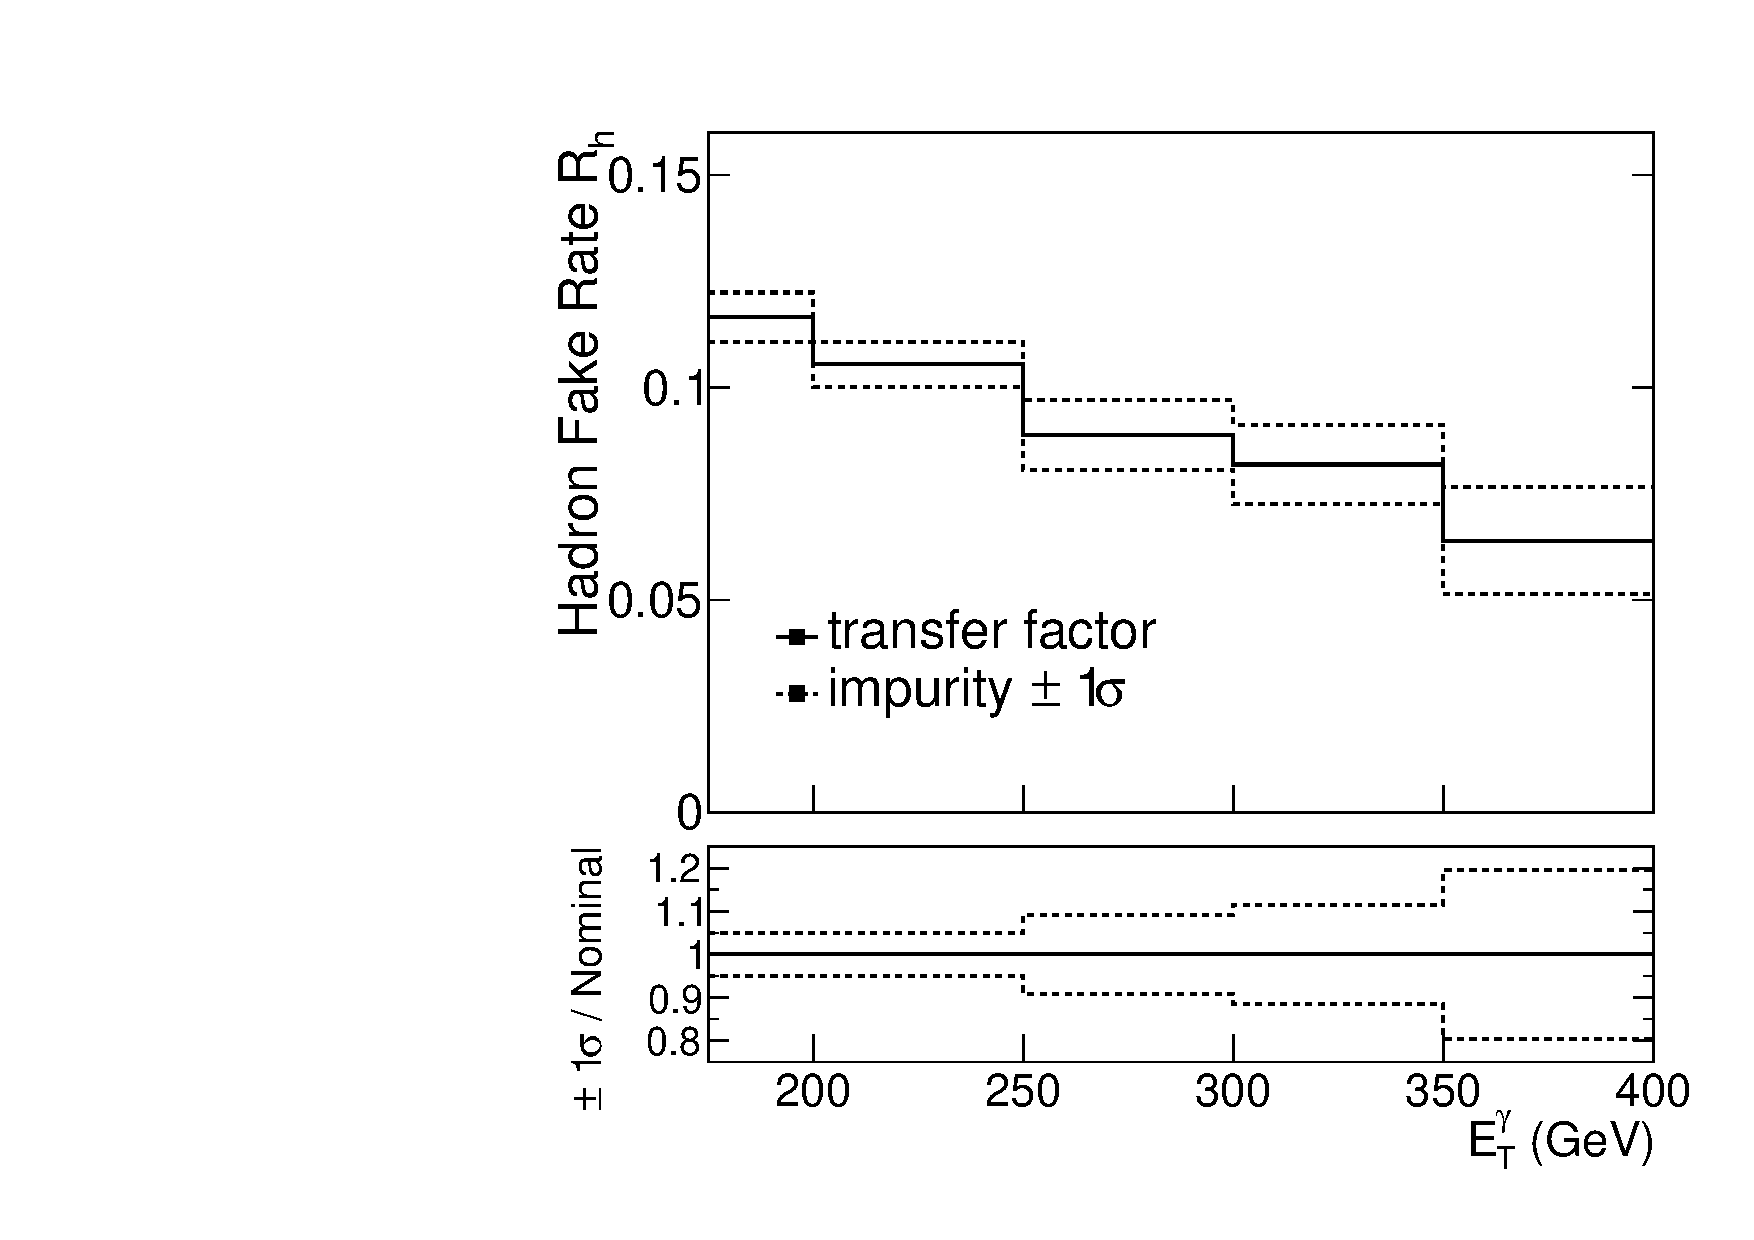
\includegraphics[]{Analysis/Figures/hfake/tfactorNom.pdf}
  }
  \resizebox{0.91\textwidth}{!}{
    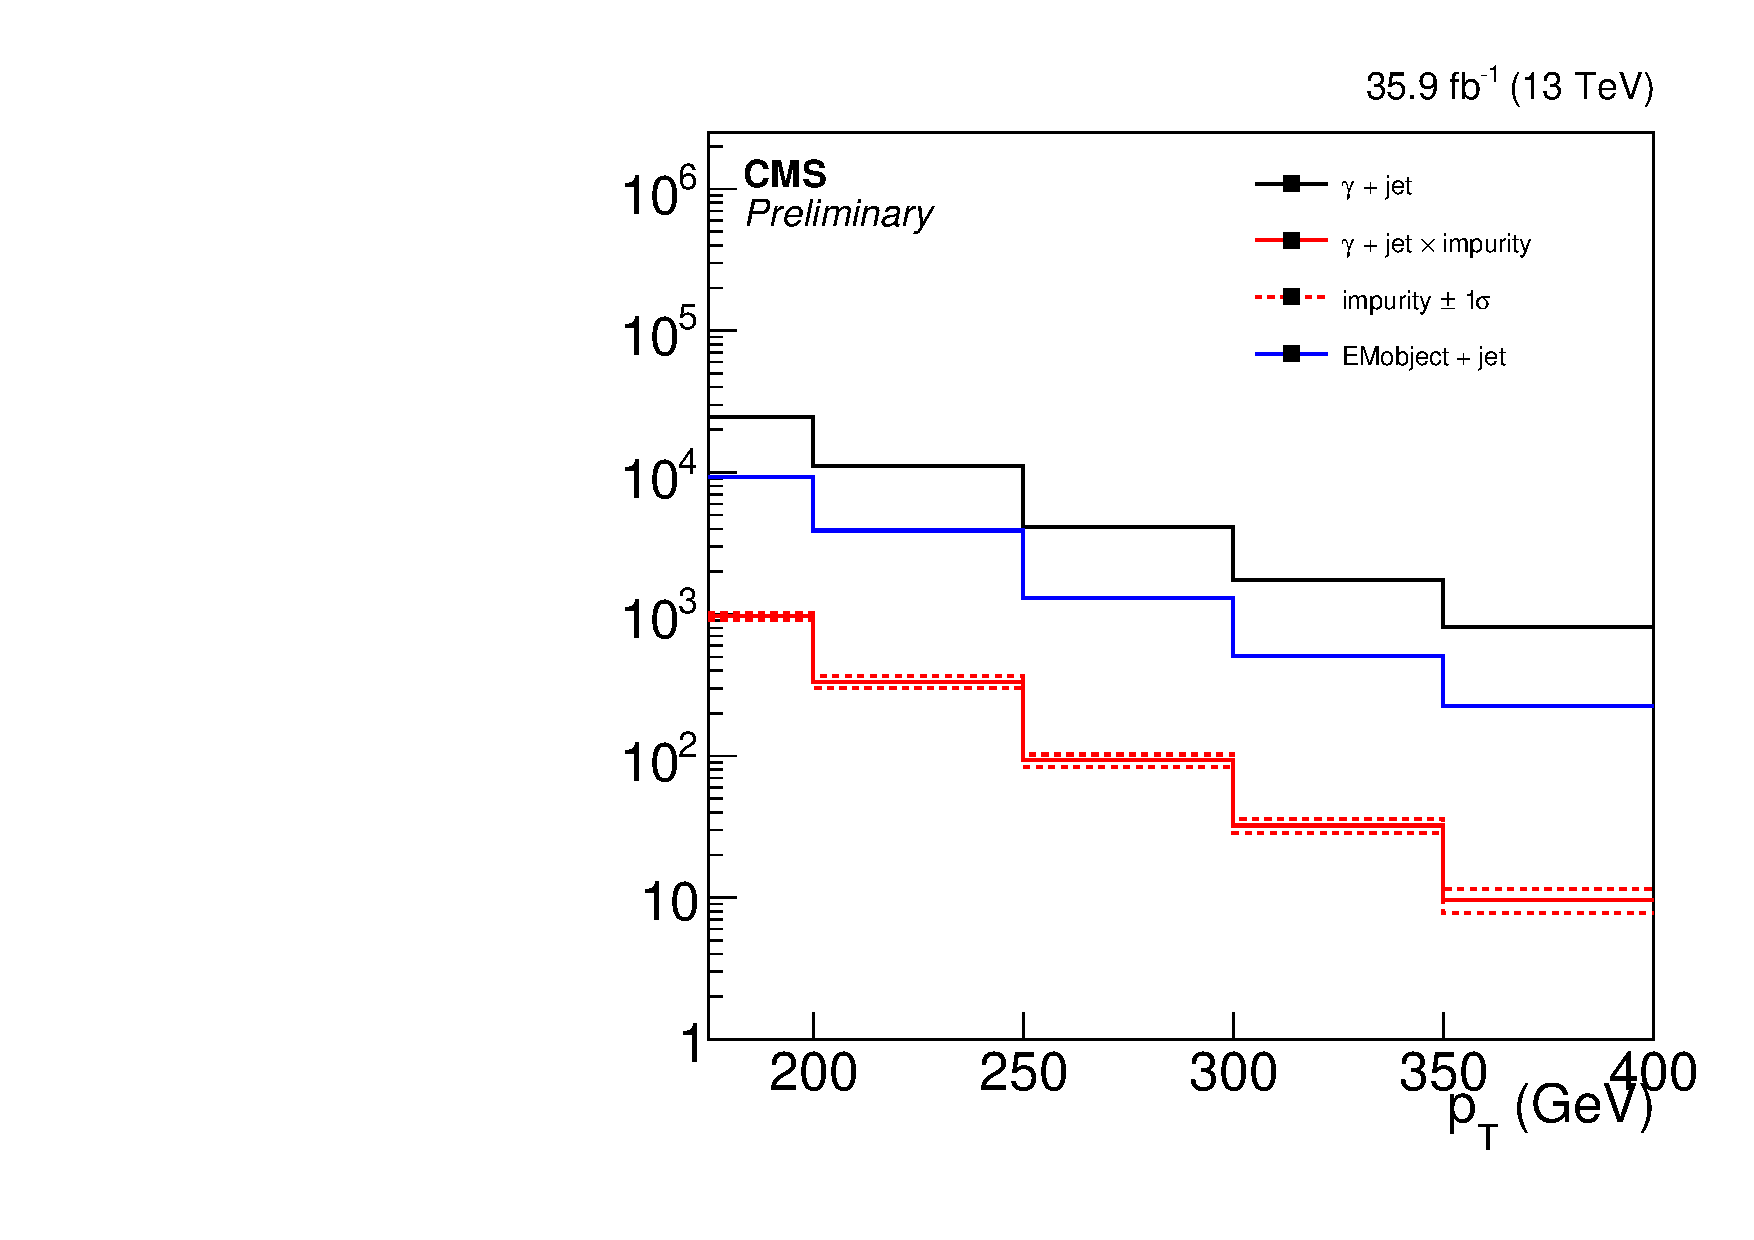
\includegraphics[]{Analysis/Figures/hfake/distributionsTight.pdf}
    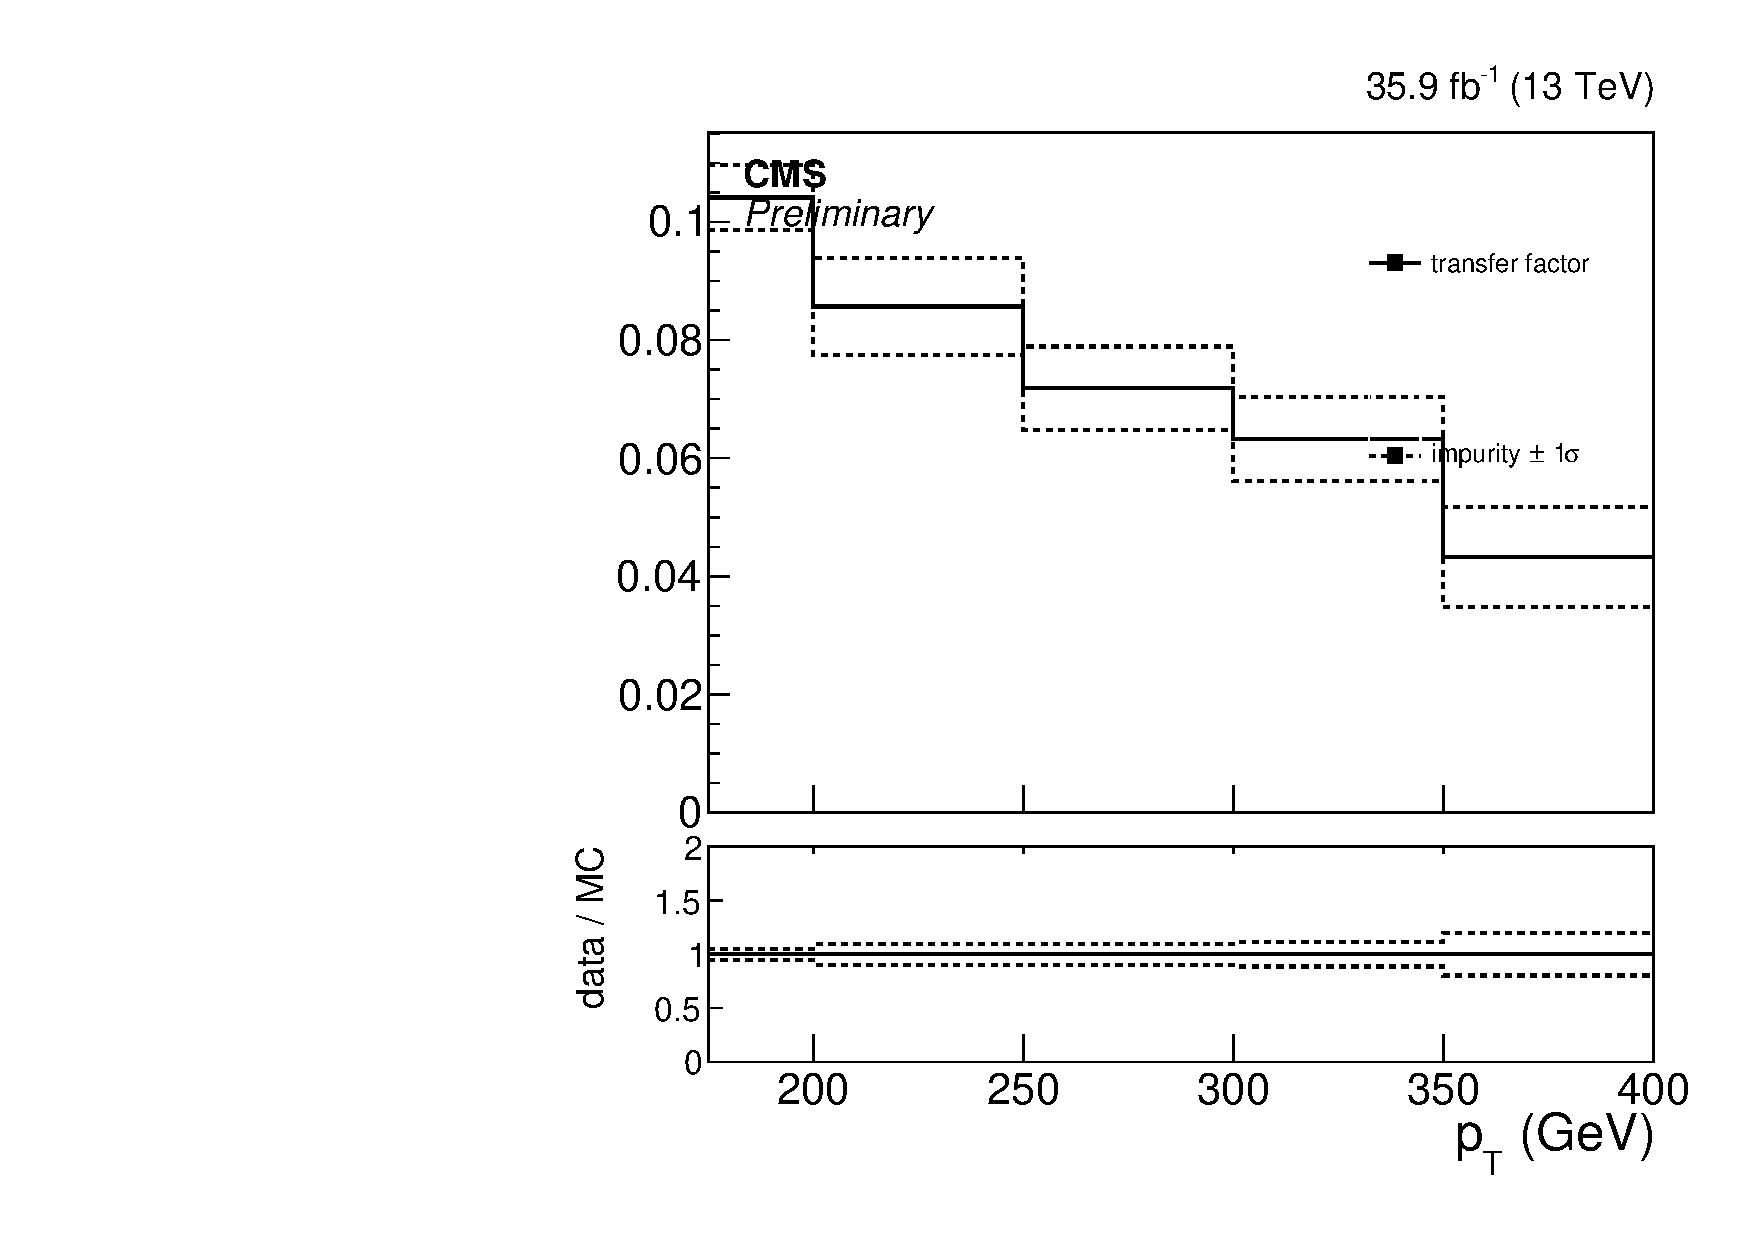
\includegraphics[]{Analysis/Figures/hfake/tfactorTight.pdf}
  }
  \resizebox{0.91\textwidth}{!}{
    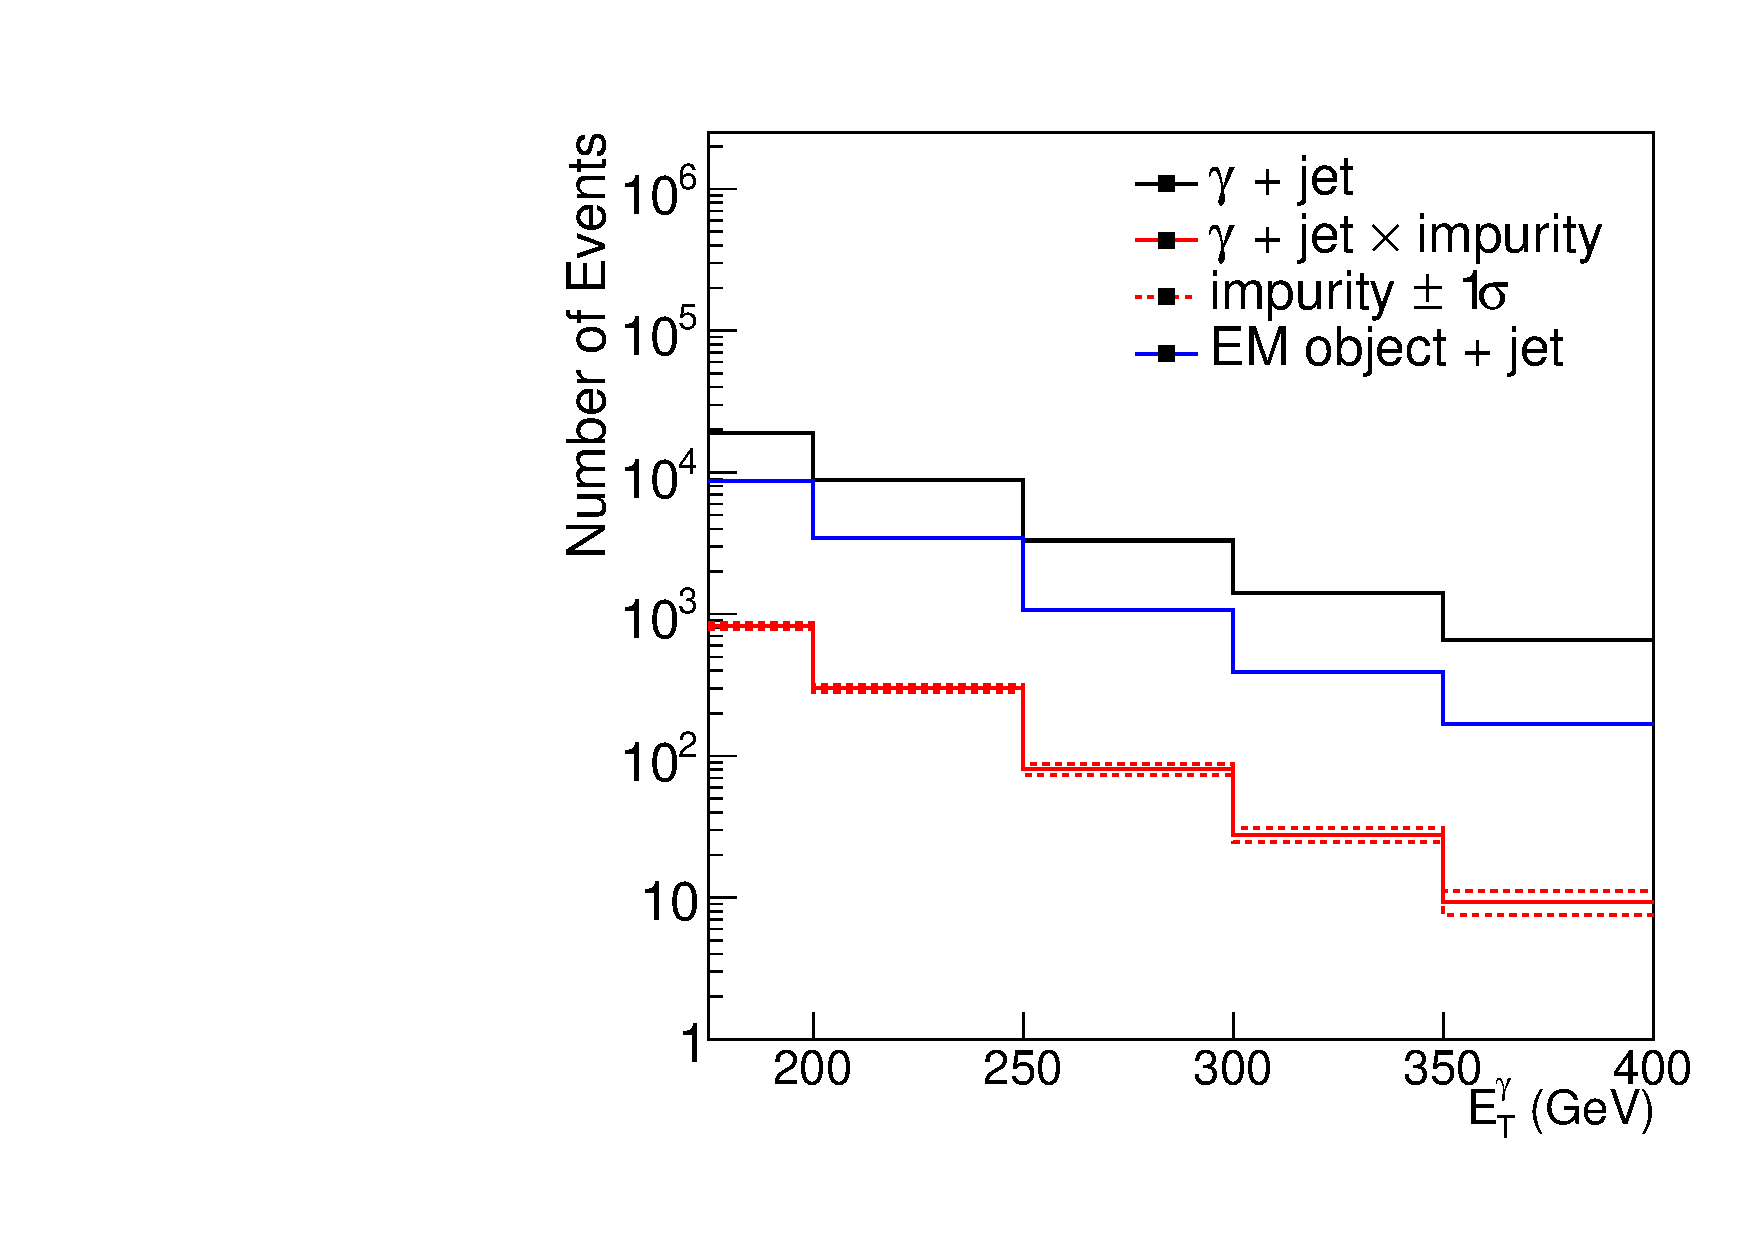
\includegraphics[]{Analysis/Figures/hfake/distributionsLoose.pdf}
    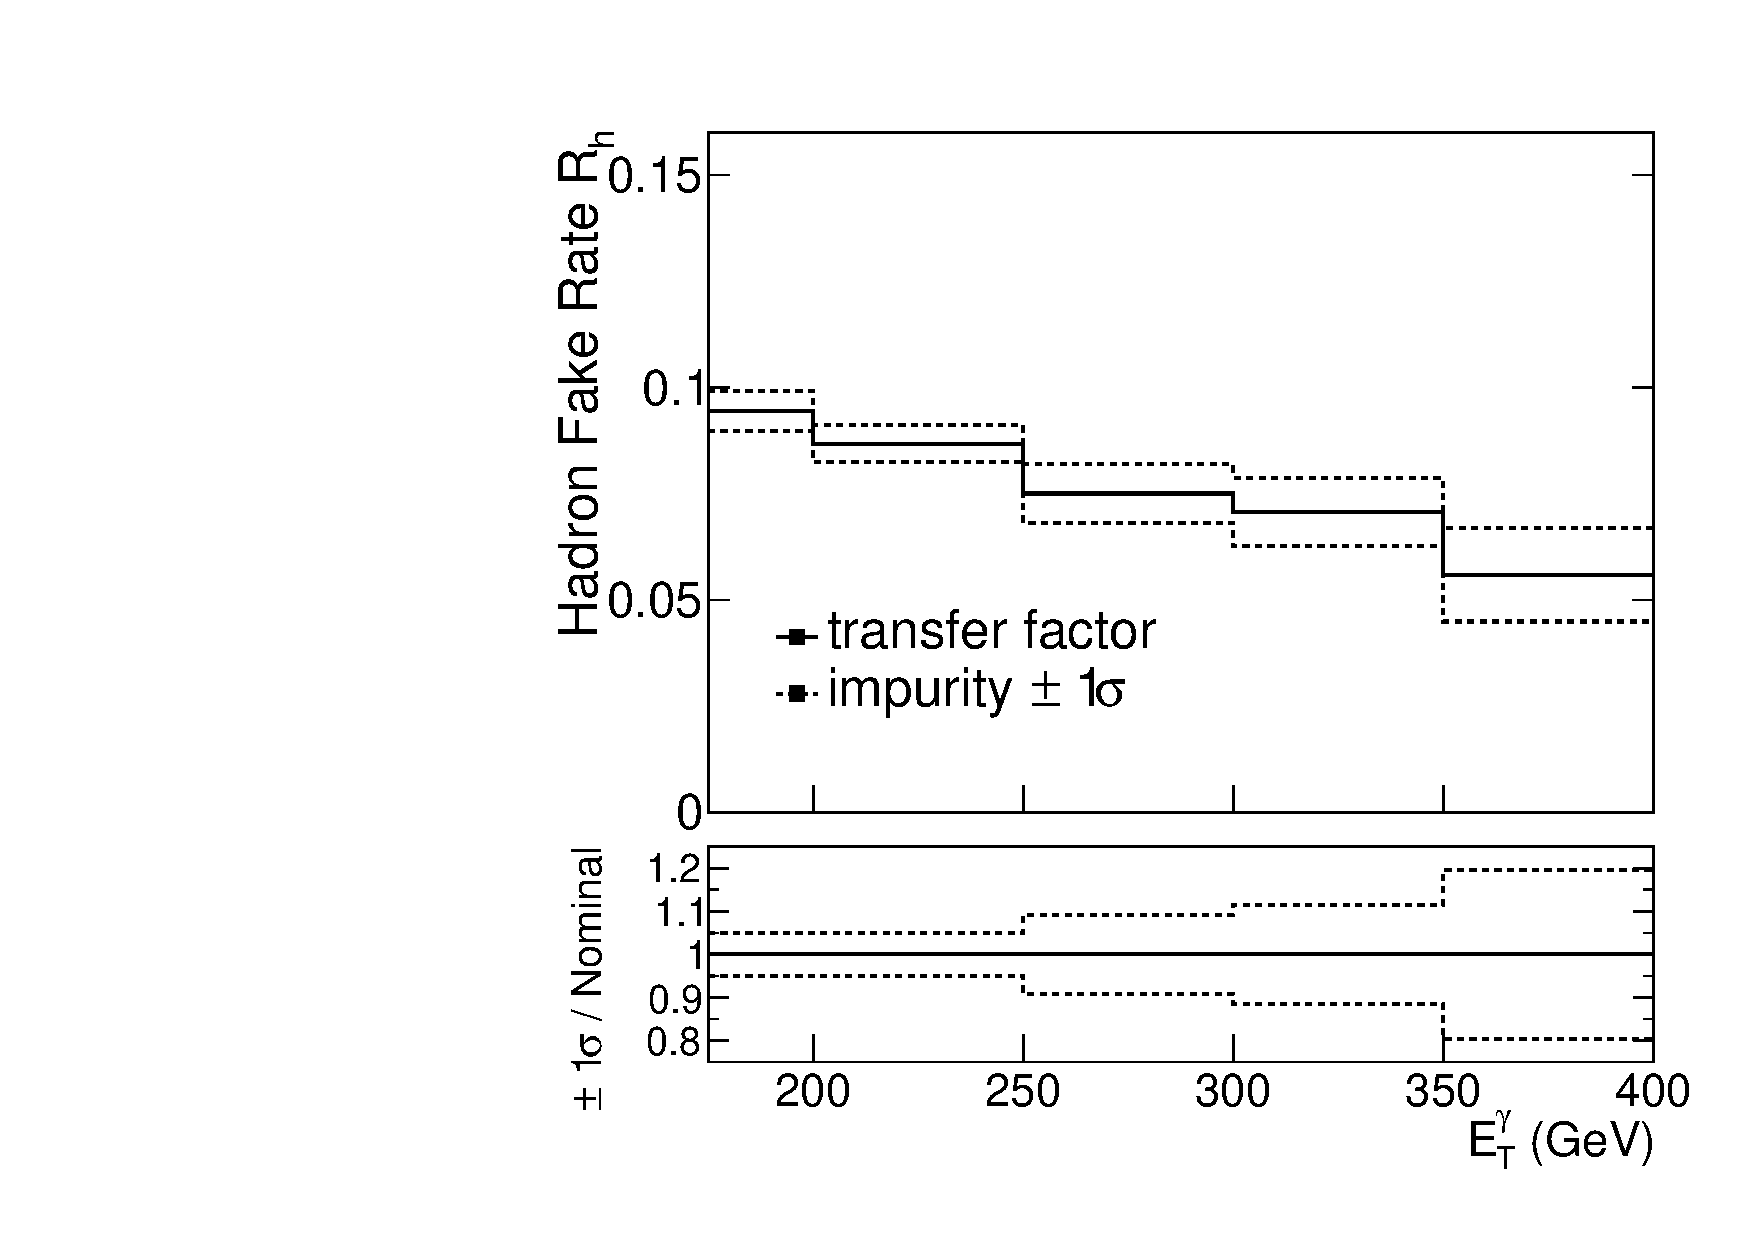
\includegraphics[]{Analysis/Figures/hfake/tfactorLoose.pdf}
  }
  \caption{
    \small Left: The \ET\ distribution of the candidate photon object in the \gj\ control sample (black), the result of scaling it with the impurity (red), and the \ET\ distribution of the hadron proxy object in the hadron proxy+jet control sample (blue).
    Right: The factor $R_{h}$, which is the ratio of the red and blue distributions in the left plot.
    The dashed bands indicate the uncertainty on $R_{h}$ due to the impurity measurement.
    Top: Nominal hadron proxy object. 
    Middle: Tighter hadron proxy object. 
    Bottom: Looser hadron proxy object.
  }
  \label{fig:hadronTFactor}
\end{figure}

To estimate the background due to misidentified hadrons, a hadron proxy+\met\ control sample is used.
This control sample is obtained by identical event selection as that of the signal region but the candidate photon is replaced by a hadron proxy object.
This yields a sample of events with similar kinematics to the signal region and well-identified proxies for misidentified hadrons.
Table~\ref{tab:proxymet} summarizes the selections for the hadron proxy+\met\ control sample. 

\begin{table}[htbp]
  \centering
    \begin{tabular}{l | l | r}
      Variable & Selection & Motivation \\
      \hline
      $\ET$ & $ > 175\GeV$ & hadron proxy object passing trigger \\
      $\abs{\eta}$ & $ < 1.44$ & match signal region kinematics \\
      \egamma\ ID & Pass all but \ICHmax\ & must be photon-like \\
      \Pgg-specific ID & Pass & must be photon-like \\
      \ICHmax\ &  $ > 1.146\GeV$ & inverted to mimic hadrons \\
      $\met $ & $ > 170\GeV$ & match signal region kinematics \\
      $\ETg / \met  $ & $ < 1.4$ & match signal region kinematics \\
      $\mindphijmet  $ & $ > 0.5$ & match signal region kinematics \\
      $\dphigmet  $ & $ > 0.5$ & match signal region kinematics \\
      Lepton Veto & Pass & match signal region \\
    \end{tabular}
  \caption{Selections for the hadron proxy+\met\ control sample.}
  \label{tab:proxymet}
\end{table}

Under the assumption that the factor $R_{h}$ stays constant regardless of whether the event has a high-\pt\ jet or \met, the hadron proxy+\met\ control sample is weighted by $R_{h}$ to determine the number of events due to misidentified hadrons in the signal region.

To estimate the uncertainty on this background, we repeat the above method using the additional tight and loose proxy definitions and corresponding control samples.
%% The different distributions from the nominal, tight, and loose selections are shown in Figure~\ref{fig:hadronFakeShapes}. 
The tight and loose shapes are taken as the one sigma band around the nominal estimate. 
Additionally, there is an uncertainty coming from the estimation of the photon purity, with values given in Table~\ref{tab:hfake-impurity-systs}. 
% Figure~\ref{fig:hadronFakePurity} shows the resulting shapes from moving the shapes generated by a one sigma shift in the purity.
